\documentclass[12pt,a4paper]{article}
% Formatação acadêmica: A4, fonte 12, margens 2,5 cm e espaçamento 1,5.
\usepackage[utf8]{inputenc}
\usepackage[T1]{fontenc}
\usepackage[brazil]{babel}
\usepackage{lmodern,microtype}
\usepackage{geometry}
\usepackage{graphicx,float,booktabs,array,longtable,tabularx,multirow}
\usepackage{xcolor,setspace,hyperref,caption,enumitem,amsmath,etoolbox}
\geometry{margin=2.5cm}
\onehalfspacing
\hypersetup{colorlinks=true,linkcolor=blue,urlcolor=blue,citecolor=blue,
 pdftitle={Tech Challenge - IA Aplicada à Saúde - Fase 4},pdfauthor={Equipe Tech Challenge FIAP}}
\setlist[itemize]{leftmargin=1.2cm}
\setlength{\emergencystretch}{3em}
\setcounter{tocdepth}{2}
\definecolor{navy}{gray}{0}
\definecolor{teal}{gray}{0}
\definecolor{light}{gray}{0.96}
\definecolor{muted}{gray}{0.25}
\newcommand{\code}[1]{\texttt{\small\detokenize{#1}}}
\newcommand{\note}[1]{\begin{quote}\small #1\end{quote}}
\newcommand{\sectionpage}[1]{\section{#1}}
\newcolumntype{Y}{>{\raggedright\arraybackslash}X}
\newcommand{\linkdovideo}{}
% Gerado exclusivamente de evidências locais; sem credenciais.
\newcommand{\DataRelatorio}{%
11 de novembro de 2026
}
\newcommand{\ResultadoAudio}{%
A avaliação foi regenerada com partições isoladas por família de frase-base. Os valores abaixo são extraídos de \path{evidence/audio_reproducao.json}; cada partição é reportada separadamente.
\begin{center}\begin{tabular}{lrrr}\toprule
Partição & Exemplos & Acurácia & F1 macro\\\midrule
Validação & 172 & 93,60\% & 0,933\\
Teste & 176 & 86,36\% & 0,862\\
Verificação cega & 120 & 88,33\% & 0,883\\
\bottomrule\end{tabular}\end{center}

}
\newcommand{\ResultadoNuvem}{%
Modelo utilizado: \textbf{gpt-4o-mini (texto) e gpt-4o-mini-transcribe (áudio)}. Chamadas reais registradas: \textbf{18}. Custo estimado acumulado: \textbf{US\$ 0,005980}. Estado registrado: 16 chamadas concluídas; duas respostas rejeitadas sem uso na decisão; inclui reserva conservadora da primeira falha.
}
\newcommand{\ResultadoTestes}{%
Suíte \textbf{pytest Python 3.12; entrega final}: 77 verificações aprovadas, 0 falhas.

Também foram aprovadas 26 verificações parametrizadas adicionais (subtestes), registradas separadamente da contagem de testes.
}
\newcommand{\ResultadoReplay}{%
Os registros completos da reprodução e da entrega estão em \path{integracao/evidencias/entrega_final_20261111/replay.json} e \path{integracao/evidencias/entrega_final_20261111/entrega_auditoria.json}.

No monitor incremental foram processados 32 pacotes. Latência local média: 0,631 ms; percentil 95 (posto mais próximo): 0,928 ms; máxima: 4,598 ms. O intervalo inclui detector estatístico, fusão e SQLite, conforme a instrumentação do monitor.
}
\newcommand{\ResultadoIntegracao}{%
Áudio novo-03, modelo congelado de treino, transcrição e análise textual reais do mesmo WAV, novo YOLO em montagem de teste e três fontes estruturadas sintéticas. Reserva por clipe apresentada separadamente, com seus eventos não detectados. No caso integrado, a confiança acústica do áudio novo-03 é 0,595, inferior ao limiar 0,70. A fonte de áudio fica inconclusiva e a cobertura permanece incompleta; o alerta alto do vídeo é preservado. Não se declara cobertura completa por terem sido fornecidos todos os arquivos.
}
\newcommand{\ResultadoRecursos}{%
GPU local NVIDIA RTX 2060: áudio anterior e novo YOLOv8s. Treino e inferência encerrados. Nenhuma sessão Colab foi iniciada. GPU utilizada nesta consolidação: sim. Sessão de computação encerrada ao final: sim.
}
\newcommand{\ResultadoMidias}{%
Foram criadas seis sínteses novas: duas referências e uma gravação reservada por voz. Não há hashes compartilhados com o corpus de 1.180 WAVs nem com as seis provas externas anteriores. O classificador emocional permaneceu congelado e não participou destes critérios.

\begin{center}\small\begin{tabular}{llcc}\toprule Voz & Cenário & Esperado & Obtido\\\midrule

Daniel & Original & Sem sinal & Sem sinal\\

Daniel & Volume reduzido & Sem sinal & Sem sinal\\

Daniel & Pausas inseridas & Sinal & Sinal\\

Daniel & Silêncio & Inconclusivo & Inconclusivo\\

Maria & Original & Sem sinal & Sem sinal\\

Maria & Volume reduzido & Sem sinal & Sem sinal\\

Maria & Pausas inseridas & Sinal & Sinal\\

Maria & Silêncio & Inconclusivo & Inconclusivo\\

\bottomrule\end{tabular}\end{center}

A versão interrompida insere 380 ms de silêncio a cada bloco de 180 ms. A versão com ganho reduzido multiplica a amplitude por 0,35. São perturbações técnicas, sem rótulo de doença; as derivações da mesma fonte não são observações independentes.

Dois vídeos geométricos novos passaram pelos cálculos reais de fluxo óptico: o controle não gerou eventos e o cenário alterado gerou 2. Não foi usado oráculo de caixas ou classes. Na montagem recebida foram processados 570 quadros e não houve aumento persistente que atingisse essa regra. Isso não significa ausência de eventos clínicos.

A reprodução contínua no ritmo original analisou 89 pares de quadros em 17,83 s de parede. Foram avaliadas 3 janelas de voz e persistidas 6 transições com sinais. O percentil 95 de processamento foi 15,20 ms por passo, além da espera da janela de cinco segundos. Não inclui ASR, nuvem ou captura clínica.

Evidência: \path{evidence/midias_complementares.json}. Nenhuma chamada paga foi feita nesta complementação.
}
\newcommand{\ResultadoVideoNovo}{%
A nova execução utilizou YOLOv8s, resolução de 416 por 416 pixels, batch 8, até 80 épocas e paciência 20. Foram concluídas 80 épocas, em 27,12 minutos de treinamento na GPU NVIDIA GeForce RTX 2060. A seleção usa somente a validação do primeiro prefixo de clipe.

\begin{center}\small\begin{tabular}{lrrr}\toprule Conjunto & Imagens & mAP50 & mAP50--95\\\midrule

Validação & 74 & 0,941 & 0,620\\

Teste & 37 & 0,980 & 0,615\\

Reserva de clipe & 60 & 0,613 & 0,299\\

\bottomrule\end{tabular}\end{center}

As métricas acima pertencem à nova execução e não são diretamente comparáveis ao mAP50 histórico: partições, preparação de anotações, batch e ambiente são diferentes. A queda de mAP50 do teste (mesmo prefixo do treino) para a reserva mostra que o valor alto no desenvolvimento não se mantém na outra origem disponível. Isso é compatível com diferenças de domínio e similaridade temporal, sem identificar uma causa única. A reserva não participou do treino, da escolha de limiares ou do checkpoint. O resultado entre prefixos não é validação em pacientes independentes.

Precisão e recall presentes no JSON são resumos de objetos da avaliação padrão Ultralytics. Não são os índices da regra temporal com limiares 0,4/0,6, cuja referência e resultados são registrados separadamente.

\begin{figure}[H]\centering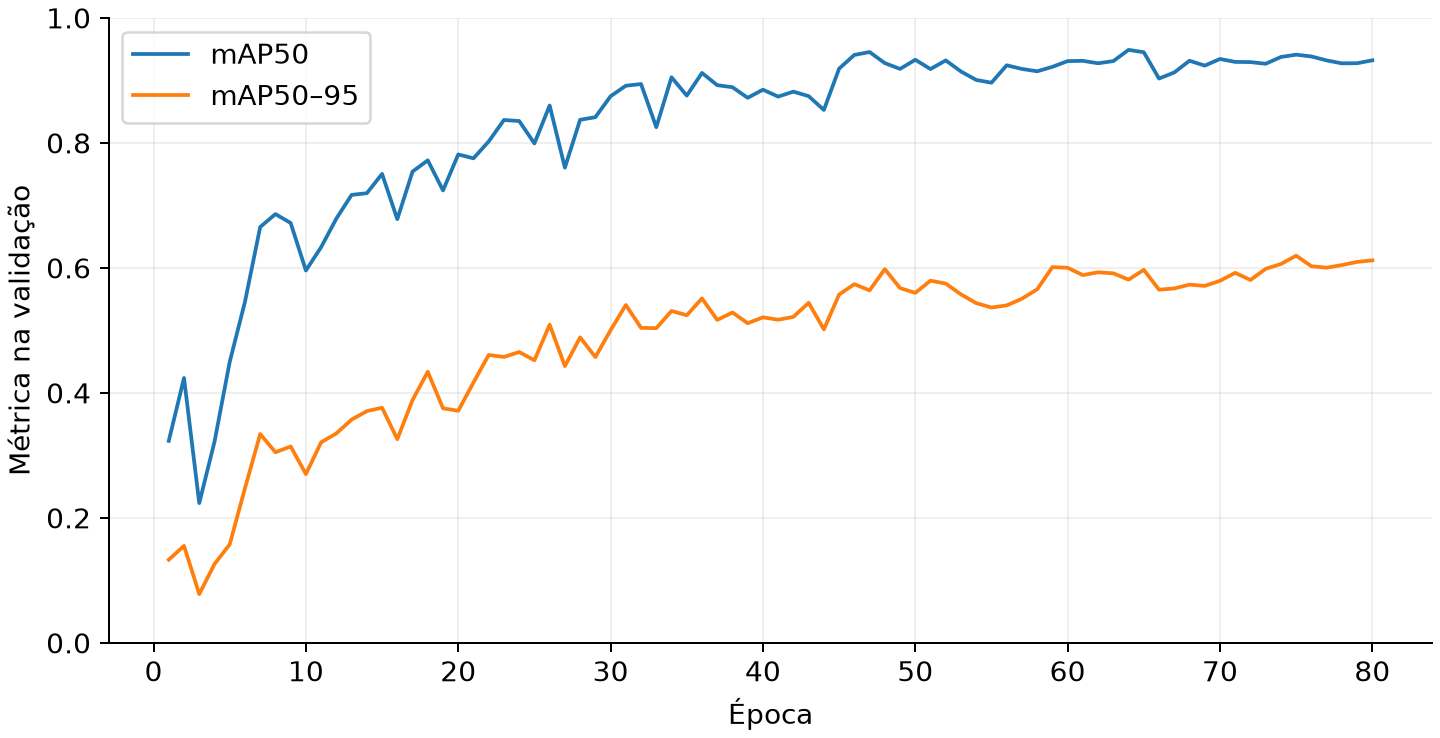
\includegraphics[width=0.92\textwidth]{figures/video_treino.png}\caption{Evolução da validação no novo treino YOLOv8s; a reserva de clipe não participa da curva.}\end{figure}

O peso congelado possui SHA-256 iniciado por \texttt{efe5cc2588300eea}. Evidências em \path{evidence/video_reproducao.json} e \path{evidence/video_dataset_auditoria.json}.

A montagem reservada foi construída após congelar o modelo, com 60 quadros-fonte não usados no desenvolvimento e duração de 120,0 segundos. A inferência gerou 0 evento(s). A referência temporal deriva das caixas anotadas e da própria regra de montagem; não é anotação clínica de complicações. A integração usa o teste para o exemplo positivo e mantém a reserva como verificação separada, sem ocultar seus eventos não detectados.

\begin{center}\small\begin{tabular}{lrrrr}\toprule Montagem & Referência & Sinalizados & Corretos & Não detectados\\\midrule

Teste & 3 & 2 & 2 & 1\\

Reserva & 2 & 0 & 0 & 2\\

\bottomrule\end{tabular}\end{center}

Os eventos são pareados uma única vez com IoU temporal de pelo menos 0,5. No teste, dois de três eventos foram recuperados (precisão 1,00 e recall 0,667). Na reserva, os dois eventos de referência não foram detectados: recall 0 e precisão não definida, pois não houve previsão positiva. A avaliação evidencia uma limitação de generalização da regra com o novo detector. Os limiares não foram ajustados depois de observar essa reserva.
}
\newcommand{\ComandosReproducao}{%
\begin{enumerate}
\item Preparar Python e instalar as dependências descritas no README.
\item Executar \code{python -m pytest -q} para a suíte de software.
\item Executar \code{python scripts/run_demo.py --help} para conferir entradas e diretório de saída.
\item Informar o CSV regenerado, o JSON de vídeo e o resultado textual real ao script de demonstração.
\item Abrir o painel com \code{python -m techchallenge4.dashboard --help} e selecionar o banco gerado.
\item Compilar o relatório com \code{python relatorio/gerar_relatorio.py --compile --package} ou importar o ZIP no Overleaf.
\end{enumerate}
}
\newcommand{\ManifestoEvidencias}{%
\small\begin{longtable}{p{8.7cm}p{4.4cm}}\toprule
Artefato & SHA-256 (prefixo)\\\midrule\endhead
\path{evidence/video_dataset_auditoria.json} & \texttt{8f14126d114c5190}\\
\path{evidence/video_reproducao.json} & \texttt{e267cdb305d3734d}\\
\path{evidence/video_inferencia_nova.json} & \texttt{30b88d7ec6fc141a}\\
\path{artifacts/video/manifesto_video.json} & \texttt{ca6187addfca1461}\\
\path{evidence/midias_complementares.json} & \texttt{4a1ad23c210416af}\\
\path{evidence/padrao_relatorio.json} & \texttt{dce7f0f2b99dd414}\\
\path{evidence/audio_reproducao.json} & \texttt{eec78c6135392737}\\
\path{audio/evidencias/particoes_audio.csv} & \texttt{30dc41d77d9167b3}\\
\path{audio/evidencias/predicoes_avaliacao.csv} & \texttt{a6b46c44b1312d97}\\
\path{artifacts/audio/manifesto_audio.json} & \texttt{fafd4dbbe961e037}\\
\path{evidence/resumo_execucao.json} & \texttt{7c9db7bb48fd5af2}\\
\path{evidence/audio_externo_transcricoes.json} & \texttt{8da6101b626df962}\\
\path{evidence/asr_comparacao.json} & \texttt{c86c4ff64c6c6263}\\
\path{evidence/audio_externo.json} & \texttt{20d055c33a303003}\\
\path{evidence/audio_recebido_drive.json} & \texttt{99a156e55c61acef}\\
\path{evidence/openai_validacao.json} & \texttt{9e43f13d89c3dc42}\\
\path{evidence/video_validacao.json} & \texttt{17832e5417cf354e}\\
\path{evidence/dashboard_validacao.json} & \texttt{e994518026d1aa81}\\
\path{integracao/evidencias/monitoramento_final/monitoramento_resumo.json} & \texttt{20c95ef1eec67a2b}\\
\path{integracao/evidencias/entrega_final_20261111/replay.json} & \texttt{8d1fc82c0db89420}\\
\path{integracao/evidencias/entrega_final_20261111/entrega_auditoria.json} & \texttt{70822b703e34beeb}\\
\path{integracao/evidencias/entrega_final_20261111/anomalias_estruturadas.json} & \texttt{e5e6f55892ed79b8}\\
\bottomrule\end{longtable}\normalsize
Os hashes completos devem ser consultados nos manifestos de execução e no histórico do repositório. O prefixo serve como referência de leitura, não como substituto de uma verificação integral.
}

\title{\textbf{Tech Challenge -- IA Aplicada à Saúde -- Fase 4}\\
\large Monitoramento Multimodal: Análise de Voz e Vídeo, Detecção de Anomalias e Alertas com IA em Nuvem}
\author{Marcelo Viana de Araujo -- RM372707\\
Nirton Afonso de Oliveira Filho -- RM370221\\
Valkiria Nonato de Faria -- RM373256\\
Benicio Antonio Cardoso -- RM371527\\\\
Pós-Graduação em IA para Devs}
\date{2026}
\begin{document}
\maketitle
\begin{center}
\textbf{Repositório GitHub da Fase 4:}\\
\url{https://github.com/Val-Faria/TechChallengeFase4/tree/Nirton}

\vspace{0.2cm}
\textbf{Dataset de vídeo -- Uterus v4:}\\
{\footnotesize\url{https://universe.roboflow.com/machinelearning-yekk6/uterus-qn1he/dataset/4}}

\ifdefempty{\linkdovideo}{}{\vspace{0.2cm}
\href{\linkdovideo}{Vídeo de demonstração}}
\end{center}
\newpage
\begingroup\singlespacing\tableofcontents\endgroup
\newpage
\section{Resumo}
Este trabalho apresenta um protótipo de monitoramento multimodal voltado à saúde da mulher. A solução combina análise de voz, detecção de objetos em vídeo, interpretação textual em nuvem e acompanhamento de sinais vitais, prescrições e movimentação. As saídas convergem para um contrato comum que conserva a origem, a prioridade e a disponibilidade de cada modalidade. Os sinais são registrados em uma caixa local de revisão, com relatórios automáticos e confirmação de leitura.

O módulo de áudio utiliza Whisper, Librosa e Random Forest sobre um corpus sintético de 1.180 gravações. O módulo de vídeo emprega YOLOv8s e uma regra temporal de visualização da área crítica. A análise textual utiliza a API da OpenAI, conforme a alternativa de fornecedor autorizada pelo professor. O monitoramento estruturado utiliza referências anteriores e estatística robusta. Os resultados demonstram a execução do fluxo e identificam limitações de generalização: as fontes não são pareadas por paciente, o áudio é sintético e a referência temporal do vídeo depende de anotações cuja exaustividade não foi confirmada.

\textbf{Palavras-chave:} análise multimodal; voz; visão computacional; anomalias; monitoramento; revisão humana.

\section{Introdução e objetivos}
O Tech Challenge da Fase 4 propõe analisar dados médicos multimodais para identificar alterações e encaminhá-las à equipe responsável. O projeto reúne processamento de áudio e vídeo, análise textual gerenciada, detecção de anomalias e entrega de alertas. O recorte adotado pela equipe combina laparoscopia ginecológica e análise observacional da voz.

São objetivos do trabalho: processar as modalidades por componentes reutilizáveis; identificar eventos e alterações temporais; integrar a análise textual em nuvem; preservar a rastreabilidade dos resultados; e demonstrar o percurso entre a observação, o alerta e sua revisão. O sistema é um protótipo acadêmico e não altera tratamentos ou condutas.



\section{Arquitetura da solução}
Áudio e vídeo são mantidos em módulos separados; contratos, detectores, persistência e painel pertencem ao pacote \code{src/techchallenge4}. Os notebooks utilizam esse código, sem duplicar as regras de decisão. Os scripts permitem reproduzir extração, avaliação e geração de relatórios.

\begin{figure}[H]
\centering
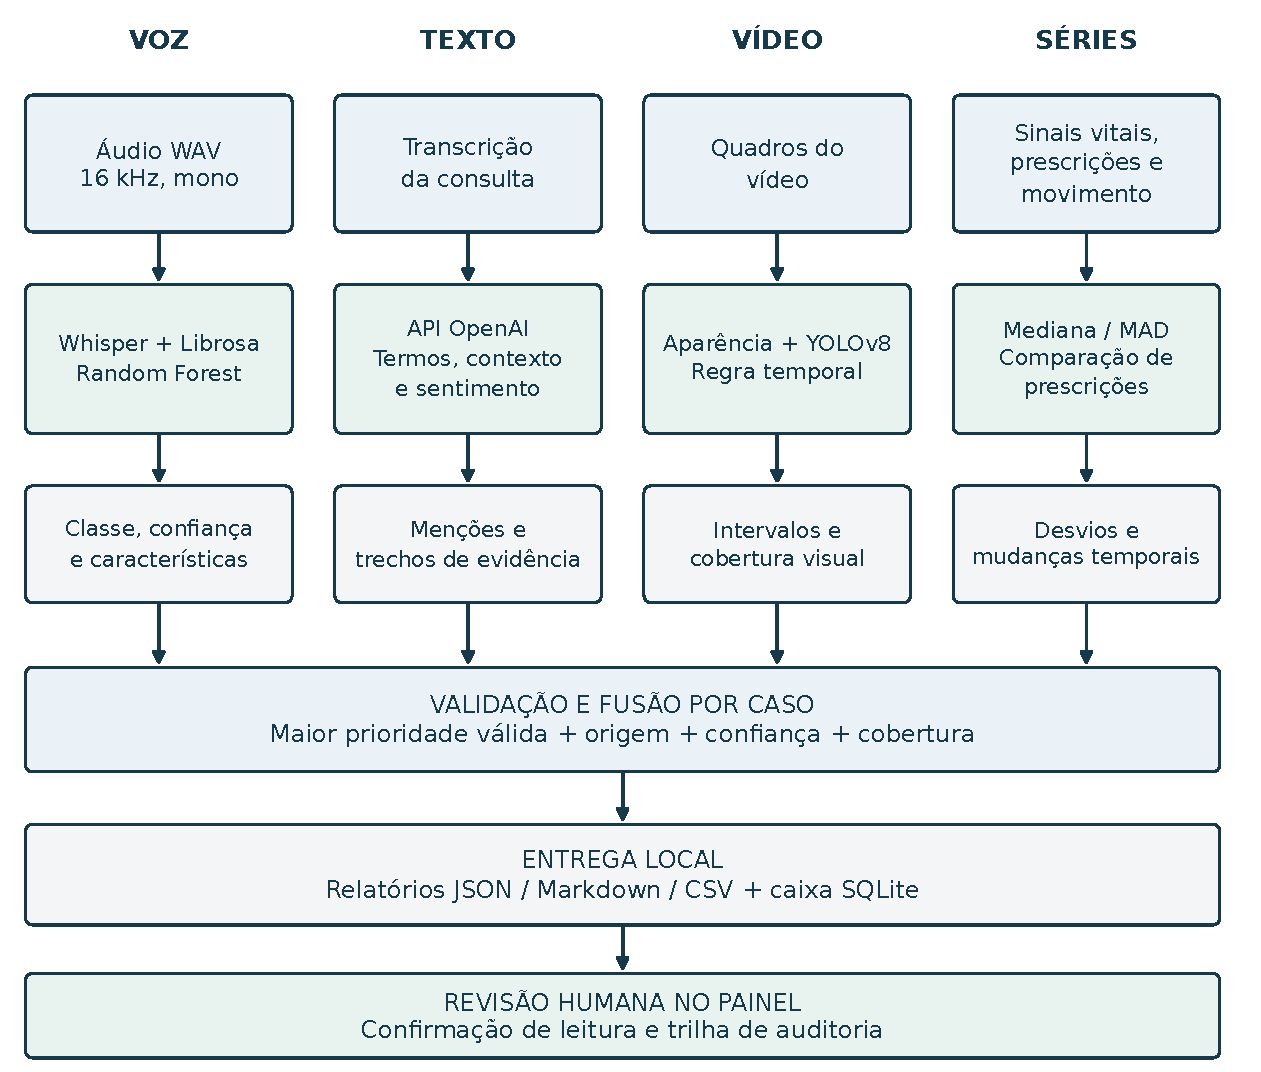
\includegraphics[width=\linewidth]{figures/fluxo_multimodal.pdf}
\caption{Fluxo multimodal: cada modalidade produz evidências que convergem para a fusão e a caixa de revisão. A transcrição da voz alimenta a análise textual; as fontes do experimento são associadas por caso e não representam um paciente pareado.}
\end{figure}



A fusão conserva a maior prioridade entre os sinais válidos. Uma modalidade neutra não cancela um alerta de maior gravidade. Fonte ausente, baixa confiança e cobertura parcial continuam identificadas e solicitam revisão. A associação das modalidades é didática, sem sincronização de um paciente real.

\section{Dados e protocolo experimental}
\subsection{Áudio e separação por frases}
O corpus contém 1.180 WAVs: 380 de ansiedade/hesitação, 400 neutros e 400 de tristeza. São 295 gravações originais, cada uma com quatro versões: original, lenta, rápida e com ruído. As falas foram produzidas por síntese de voz; seus rótulos representam as condições de construção do experimento.

A unidade de separação é a família de frase-base. Gravações e aumentos de uma mesma família permanecem no mesmo conjunto: 712 exemplos de treino, 172 de validação, 176 de teste e 120 de reserva. Não há sobreposição de famílias, gravações originais ou hashes entre partições. O modelo avaliado foi ajustado somente no treino; o classificador anterior da equipe, treinado em todo o corpus, é histórico e não participa dessas métricas.

Além do corpus, foram produzidas seis falas com textos novos e duas vozes diferentes da voz de origem. Elas não integram o ajuste nem possuem rótulos clínicos independentes. Outras seis sínteses, distintas das anteriores, fornecem referências e controles físicos para a análise de pausas.

\subsection{Vídeo e reserva de origem}
A fonte é o Uterus Dataset v4, do Roboflow Universe. A página anuncia 1.368 imagens; o ZIP contém 1.367: 1.196 de treino, 114 de validação e 57 de teste. A preparação verifica CRC, integridade e duplicatas. As anotações misturam polígonos e caixas; 418 polígonos utilizados foram convertidos em caixas envolventes, sem criar rótulos anatômicos adicionais.

O prefixo \code{UterusClip_mov} fornece 776 imagens de treino, 74 de validação e 37 de teste. O prefixo \code{2024-09-26-20-27-33_mp4} foi excluído do desenvolvimento: suas 420 versões aumentadas não são utilizadas, e 60 imagens originais formam a reserva. A identidade de clipe inferida do nome não comprova independência por paciente. As montagens repetem cada imagem por dois segundos; seus intervalos não representam a duração original de eventos cirúrgicos.

Uma fonte complementar do TVASurg, Universidade de Toronto, foi utilizada somente para verificação qualitativa. Trata-se de um vídeo didático editado, sem referência independente de eventos clínicos. As imagens não integram o repositório ou este relatório.

\subsection{Séries e dados textuais}
Sinais vitais, prescrições e movimentação são séries sintéticas com timestamps. Elas permitem verificar ordenação, cálculo de desvios, fusão e entrega incremental. Os textos de consulta são transcrições de falas sintéticas e casos de controle com afirmação, negação e contexto histórico. As fontes disponíveis não constituem uma coorte clínica.

\section{Análise de áudio}
\subsection{Características e classificador}
Os WAVs são convertidos para mono a 16 kHz. O Whisper tiny transcreve em português; o Librosa calcula as características utilizadas pelo Random Forest.

\begin{center}\small\begin{tabularx}{\linewidth}{lY}\toprule
Característica & Cálculo\\\midrule
Duração & Quantidade de amostras dividida pela taxa de amostragem.\\
Energia média & Média da energia RMS em janelas.\\
Proporção de pausas & Fração fora dos intervalos sonoros, com \code{top_db=30}.\\
Ritmo & Palavras reconhecidas por minuto de gravação.\\
Tom médio e variação & Média e desvio padrão dos valores válidos de F0 por pYIN.\\\bottomrule
\end{tabularx}\end{center}

O Random Forest usa 200 árvores, semente 42 e ponderação balanceada de classes. Não houve busca de hiperparâmetros ou reajuste com as reservas. Na integração, confiança inferior a 0,70 permanece inconclusiva. As classes de prosódia não são diagnósticos e não demonstram, por si, detecção de fadiga, disartria ou dificuldade respiratória.

\ResultadoAudio

\begin{figure}[H]\centering
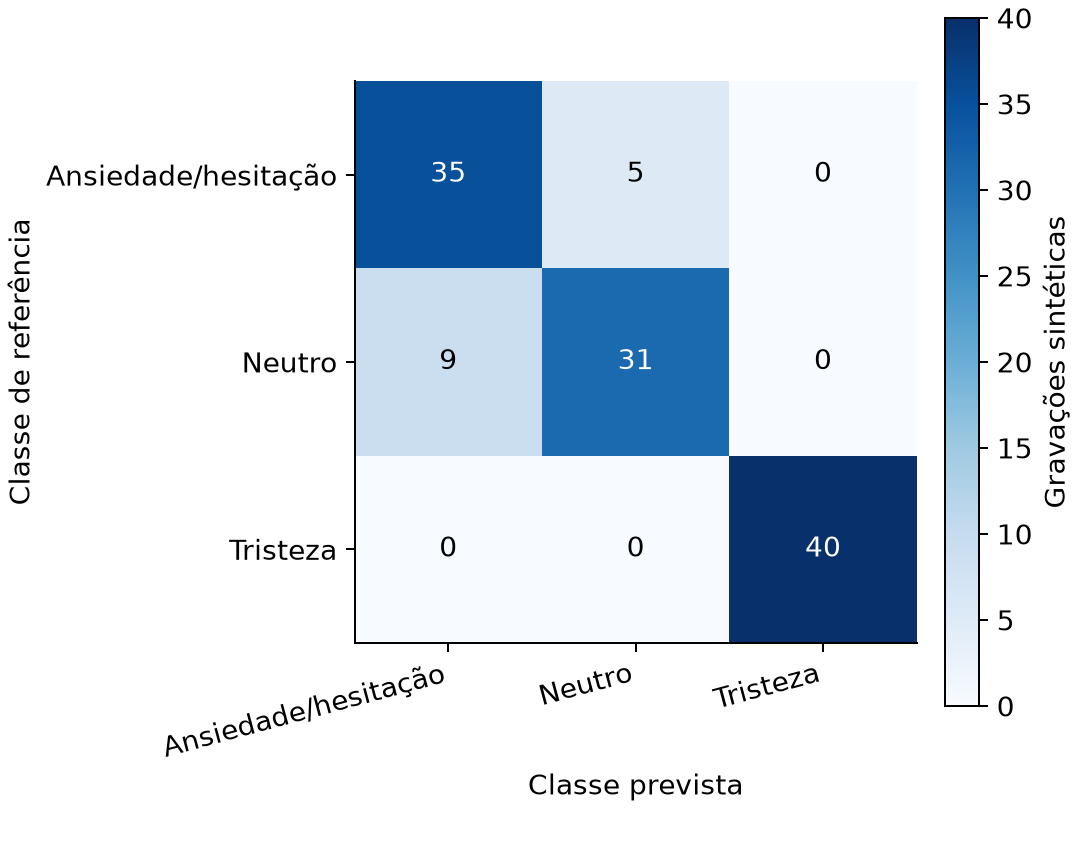
\includegraphics[width=0.75\textwidth]{figures/audio_matriz_cega.png}
\caption{Matriz de confusão da reserva de frases do classificador emocional sintético.}
\end{figure}

\subsection{Transcrição e gravações externas}
O Whisper apresentou 13 erros em 109 palavras nas seis gravações externas, WER agregado de 11,9\%. No caso novo-03, a expressão ``falta de ar'' foi transcrita como ``falta de área''. A API \code{gpt-4o-mini-transcribe} apresentou zero erros nessa pequena amostra, com os mesmos hashes de WAV e normalização textual. A comparação não estabelece superioridade geral nem desempenho em pacientes.

Todas as seis previsões acústicas externas ficaram abaixo de 0,70. Elas são encaminhadas como inconclusivas. O ritmo do classificador permanece baseado no Whisper para manter a representação do treinamento; a transcrição em nuvem alimenta a análise textual separadamente.

\subsection{Alterações vocais observacionais}
A comparação intra-voz utiliza duas gravações anteriores da mesma voz, com referência congelada antes da observação nova. Janelas RMS de 20 ms estimam atividade vocal. A regra exige aumento de pelo menos 0,20 na proporção de pausas e redução do trecho vocal mediano para até 65\% da referência. Saturação, silêncio ou duração insuficiente tornam o resultado inconclusivo. Os limites são demonstrativos e não atribuem causa médica às alterações.

\section{Análise de vídeo}
\subsection{Detector e regra temporal}
O modelo avaliado é um YOLOv8s com ajuste a partir de pesos COCO, diferente do peso original da frente de vídeo. A inferência detecta instrumentos e útero em resolução de $416\times416$ pixels. O script exige confiança mínima de 0,4 para instrumento e 0,6 para útero. Instrumento detectado sem detecção sustentada de útero por pelo menos cinco segundos gera um sinal, com tolerância de um segundo para interrupções curtas.

A prioridade é baixa a partir de cinco segundos, média a partir de dez e alta a partir de quinze, ou com pelo menos três eventos. A ausência de detecção não comprova ausência anatômica. Os sinais solicitam revisão e podem ocorrer durante etapas normais do procedimento.

\begin{figure}[H]
\centering
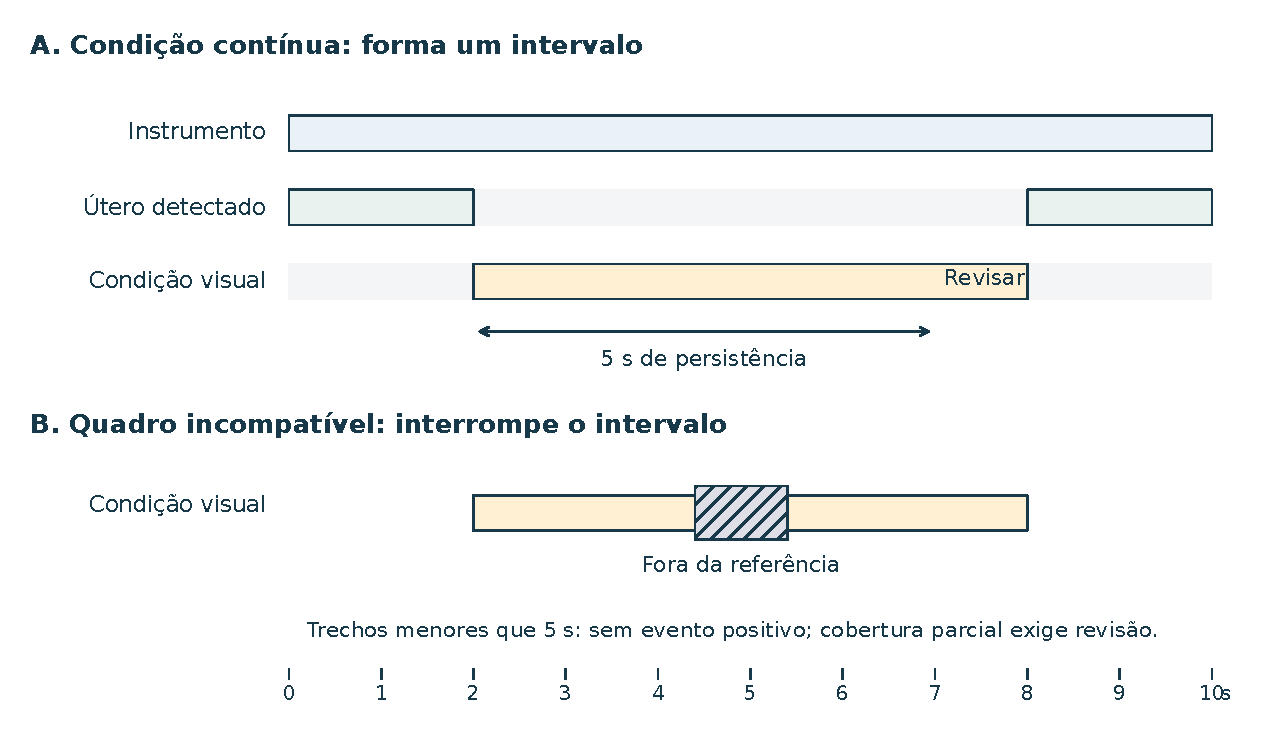
\includegraphics[width=\linewidth]{figures/regra_temporal_didatica.pdf}
\caption{Esquema ilustrativo da regra temporal, sem medir desempenho clínico. No cenário A, a condição persiste por tempo suficiente; no B, um quadro incompatível interrompe a sequência. Ausência de evento positivo não elimina a necessidade de revisão da cobertura.}
\end{figure}


\ResultadoVideoNovo

\subsection{Anotações, calibração e compatibilidade visual}
\ResultadoVideoRevisao

\subsection{Resultados históricos da equipe}
O pacote original registra uma montagem de 114 segundos, 570 quadros e dois intervalos: 76--82 e 84--114 segundos, com confiança média de 0,82 e 0,81. A regra reproduziu esses intervalos a partir das detecções recebidas. Esses registros documentam a frente original; não são métricas do novo modelo. Os índices históricos e sua descrição permanecem em \path{relatorio/secao_video.md}.

\section{Análise textual em nuvem}
A transcrição é enviada à API da OpenAI para extrair sentimento, termos relevantes, contexto e trechos literais. O fornecedor substitui os serviços Azure conforme orientação docente registrada em \path{evidence/orientacao_docente.md}. O formato estruturado é validado antes da integração.

Menções afirmadas, negadas ou incertas permanecem distintas. Contexto histórico ou de terceiros não é interpretado como sintoma atual do paciente. A existência de JSON válido não garante correção semântica; os controles incluem negação, citação e instruções conflitantes no texto. Sentimento e classe acústica não são somados como probabilidades de gravidade clínica.

\ResultadoNuvem

As chamadas usam cache, limite local de solicitações e reserva de orçamento. O custo é estimado a partir dos dados de uso, não uma consulta à fatura. As demonstrações da entrega reutilizam respostas salvas; nenhuma chave é necessária para visualizá-las. Novas chamadas são opcionais e a credencial fica em variável de ambiente ou nos Secrets do Colab.

\section{Anomalias e monitoramento temporal}
\subsection{Sinais vitais e movimentação}
Uma referência anterior de pelo menos vinte observações é congelada antes de avaliar os novos pontos. Para cada campo, utilizam-se a mediana e a escala robusta baseada no desvio absoluto mediano (MAD):
\[
 s = 1{,}4826\,\operatorname{mediana}(|x_i-\operatorname{mediana}(x)|),\qquad
 z = \frac{|x-\operatorname{mediana}(x)|}{s}.
\]
A demonstração sinaliza $z\geq6$. Referências sem dispersão suficiente permanecem inconclusivas. Os campos incluem batimentos, pressão sistólica e diastólica, oxigenação e medidas de movimentação. São limites estatísticos de demonstração, não protocolos assistenciais.

\begin{figure}[H]\centering
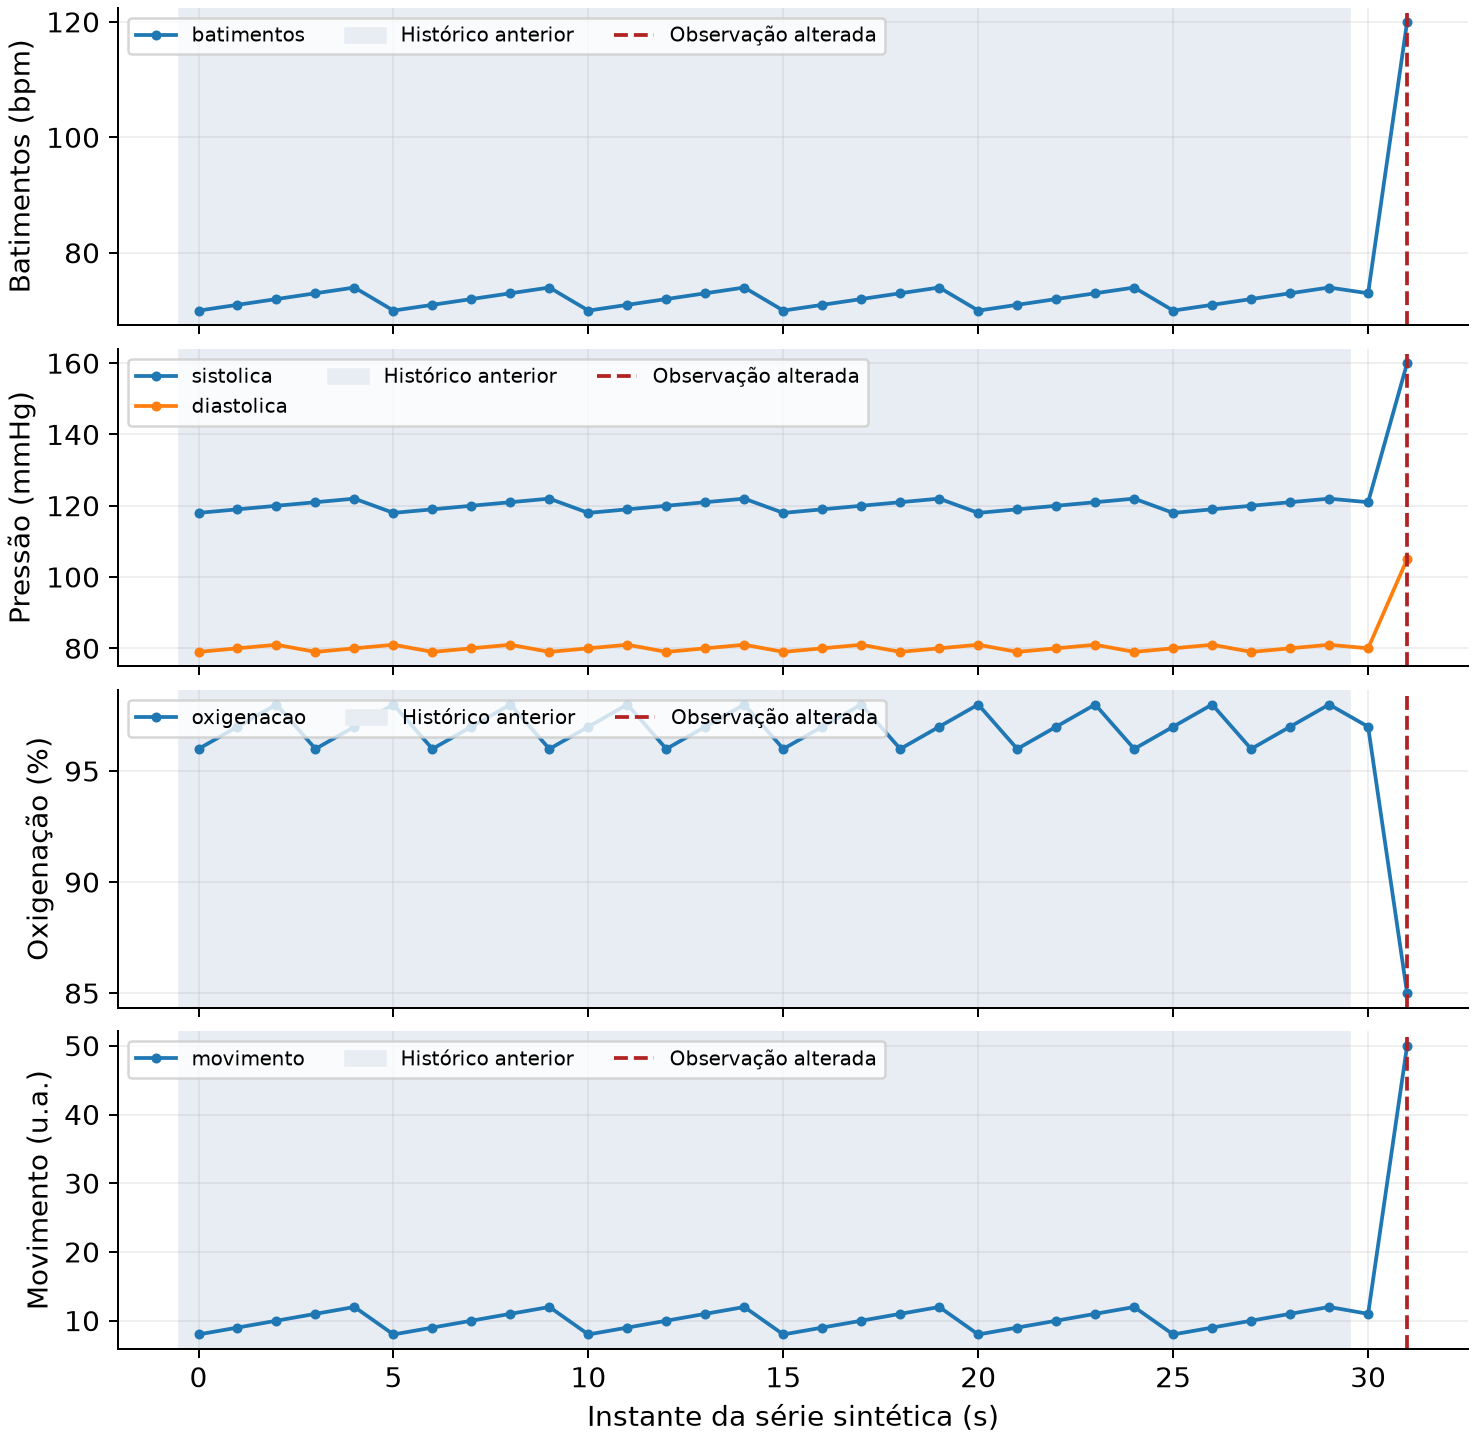
\includegraphics[width=0.9\textwidth]{figures/series_demonstracao.png}
\caption{Histórico e alterações sintéticas utilizados na avaliação do monitor estruturado.}
\end{figure}

\subsection{Prescrições}
Os registros sucessivos de um medicamento são comparados preservando unidade, via e intervalo. A variação relativa da dose só é calculada quando unidade e via são compatíveis; a demonstração sinaliza variação de pelo menos 50\%. Mudanças de unidade, via ou intervalo são descritas separadamente. O detector não recomenda doses ou alterações de tratamento.

\subsection{Inferência em mídias e latência}
O fluxo óptico denso de Farnebäck mede alterações inespecíficas de movimento entre quadros. Ele não reconhece anatomia ou postura clínica. As referências utilizam apenas observações anteriores. A execução incremental recebe JSONL ou processa amostras de áudio e quadros de arquivos no ritmo original.

\ResultadoMidias

A espera da janela de áudio é de cinco segundos. As medições locais de processamento são separadas dessa espera; não incluem reconhecimento de fala em nuvem, aquisição clínica ou rede hospitalar. A reprodução de resultados prontos mede persistência e entrega, não a inferência dos modelos.

\section{Fusão, entrega e revisão}
Cada fonte informa origem, estado, alerta, prioridade e limitações. Baixa confiança, indisponibilidade, erro e cobertura parcial são preservados. A maior prioridade válida define o nível do caso, sem cancelar a indicação de modalidades inconclusivas.

A caixa SQLite utiliza transações e uma identidade estável para impedir entregas duplicadas. A confirmação de revisão conserva o responsável e o instante em uma trilha de auditoria. Os relatórios JSON, Markdown e CSV são gravados de forma atômica. O painel HTTP se vincula a \code{127.0.0.1} e demonstra revisão local, sem comunicação com um hospital.

\ResultadoIntegracao

\begin{figure}[H]
\centering
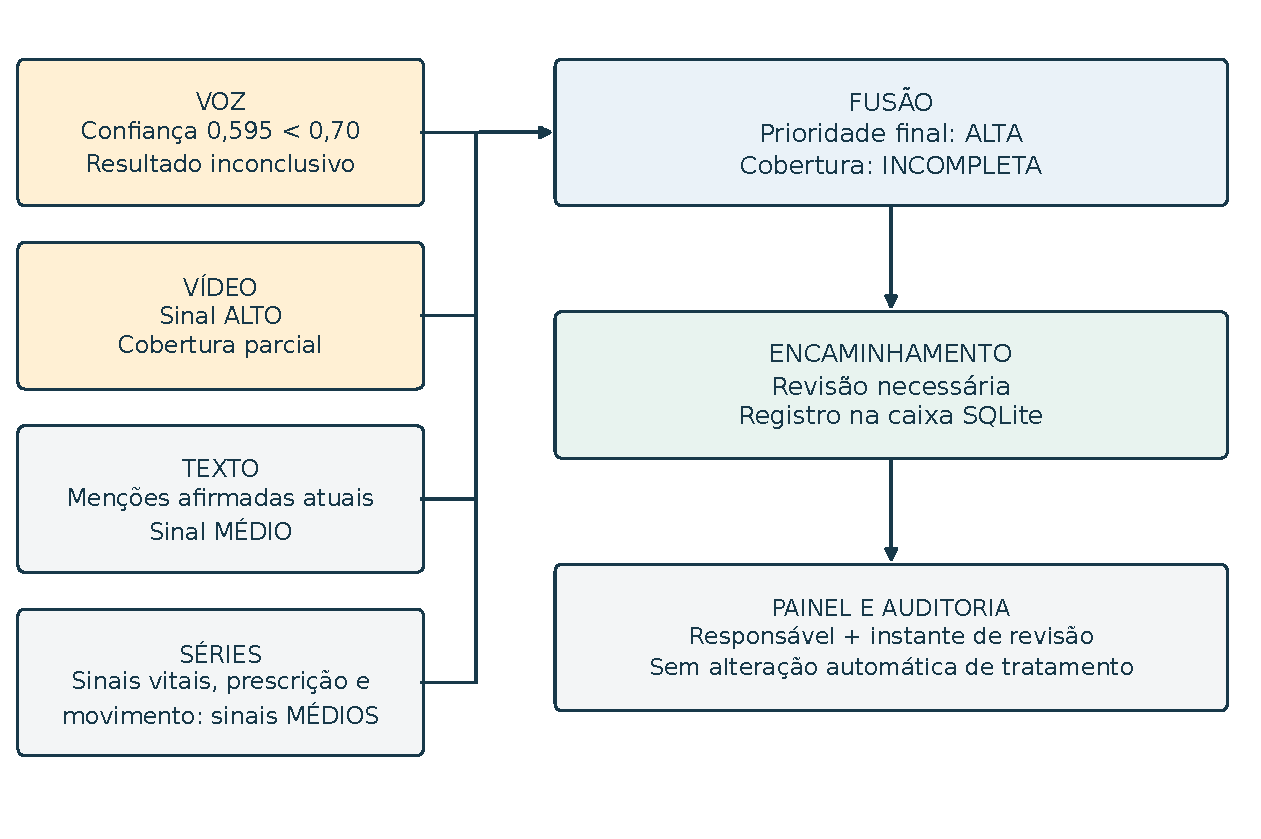
\includegraphics[width=\linewidth]{figures/exemplo_fusao.pdf}
\caption{Decisão do caso integrado registrado. O sinal alto de vídeo é preservado, enquanto baixa confiança e cobertura parcial mantêm o caso incompleto. A associação de fontes é didática e exige revisão humana.}
\end{figure}

\ResultadoReplay

Os controles também verificam vídeo sem evento positivo e com cobertura parcial: o caso permanece na fila. No controle positivo, a prioridade alta é mantida. A confirmação automática de teste é identificada como demonstração, sem atribuir revisão clínica a um profissional.

\section{Verificação e reprodução}
\ResultadoTestes

A suíte cobre contratos, prioridade, dados ausentes, validade temporal, pressão arterial, comparações de prescrições, concorrência, entrega idempotente, cache, orçamento e interrupção da regra visual. O painel foi verificado por GET e confirmação POST com persistência da auditoria. Os testes de software não substituem avaliação do desempenho clínico.

\subsection{Notebooks e ambiente}
Os três notebooks são distribuídos com saídas salvas de execução local, compatíveis com Google Colab. O notebook de áudio recalcula previsões com o modelo congelado; vídeo apresenta métricas de treinamento e inferência registradas; integração executa fusão, detectores estruturados, relatórios e painel. Gráficos e tabelas distinguem essas etapas. Não há novo ajuste ou chamada paga no modo padrão.

\ResultadoRecursos

O código está organizado em pacote comum, módulos de áudio/vídeo, scripts e testes. As partições, os hashes e as versões dos artefatos permitem repetir os experimentos. Os arquivos de entrada privados e o peso YOLO ficam no backup da equipe, com instruções de restauração em \path{DATASETS_E_MODELOS.md}. Experimentos antigos permanecem identificados como históricos.

\ComandosReproducao

\section{Limitações e conclusão}
O projeto demonstra o fluxo multimodal e a entrega local de sinais para revisão. O corpus sintético não representa diversidade de pacientes, condições médicas ou ambientes. A reserva por frase reduz similaridade textual, mas não estabelece independência de locutor. Os controles acústicos verificam pausas e trechos vocais, sem medir sensibilidade para uma condição médica.

No vídeo, os dois intervalos derivados de caixas da reserva continuam sem pareamento. A ausência de caixa anotada não confirma ausência do órgão, e uma anotação independente deve distinguir presença, ausência confirmada e visibilidade inconclusiva. A fonte didática externa não possui rótulos clínicos para calcular acurácia; a proteção de aparência corrige um falso alerta técnico, mas não comprova detecção confiável de falhas cirúrgicas.

As modalidades não são sincronizadas por paciente; valores estruturados e controles de apresentação são sintéticos. As decisões exigem contexto e revisão humana. O sistema não altera condutas, e as medições de latência não demonstram funcionamento em um hospital. Essas restrições delimitam os resultados e orientam uma avaliação futura com dados anotados de outras origens.

\clearpage
\section{Referências}
\begingroup\singlespacing\small
\begin{enumerate}[label={[\arabic*]},leftmargin=2em]
\item FIAP. \textit{IADT -- Fase 4 -- Tech challenge}. Enunciado, páginas 2--4, 2026.
\item FIAP. \textit{Análise de vídeo, áudio e texto}; \textit{Integração e automação com a API da OpenAI}. Materiais da Fase 4, 2026.
\item Machinelearning. \textit{Uterus Dataset}, versão 4. \url{https://universe.roboflow.com/machinelearning-yekk6/uterus-qn1he/dataset/4}.
\item TVASurg, Universidade de Toronto. \textit{Total Laparoscopic Hysterectomy}. \url{https://pie.med.utoronto.ca/TVASurg/project/gyn-tlh/}.
\item OpenAI. \textit{Structured model outputs}. \url{https://developers.openai.com/api/docs/guides/structured-outputs}.
\item OpenAI. \textit{Whisper}. \url{https://github.com/openai/whisper}.
\item Librosa. \textit{Feature extraction and pYIN}. \url{https://librosa.org/doc/latest/}.
\item Scikit-learn. \textit{RandomForestClassifier; model persistence}. \url{https://scikit-learn.org/stable/}.
\item Ultralytics. \textit{YOLOv8 documentation}. \url{https://docs.ultralytics.com/models/yolov8/}.
\item OpenCV. \textit{Optical Flow}. \url{https://docs.opencv.org/4.x/d4/dee/tutorial_optical_flow.html}.
\end{enumerate}
\endgroup
\clearpage
\appendix
\section{Manifesto de evidências}
\begin{spacing}{1.0}\ManifestoEvidencias\end{spacing}
\end{document}
